\documentclass{article}
\usepackage{import}
\subimport{../}{preamble}
\begin{document}

\section{Plasmon Coupling}

% Basic introduction to charge interaction and gap modes
Both the resonant field enhancement and the confinement of a surface plasmon can be improved by bringing a second plasmon into close proximity. Similar to coupled harmonic oscillators and dipoles, plasmons couple together once in close proximity. Normal modes of oscillation are formed once the charge distribution of one plasmon strongly couples via Coulomb forces with the charge distribution of an adjacent plasmon. In many cases the resulting normal mode has it's charge distribution strongly confined to the dielectric space between metallic surfaces where charges interact most. Normal modes are therefore more generally known as \emph{gap plasmons}.

Coupling between plasmons is a feature of many metallic systems with closely spaced metal-dielectric interfaces, including metal-insulator-metal (MIM) and insulator-metal-insulator (IMI) waveguides and systems containing multiple \glspl{mnp}. For the purposes of this work, further discussion is restricted to the ideal case of coupled \glspl{lsp} between two closely spaced \glspl{mnp}, though the coupling description is valid for many other cases involving \glspl{sp}.

\subsection{Localised Surface Plasmon Hybridisation in Plasmonic Nano-Gap Cavities}

\begin{figure}[bt]
\centering
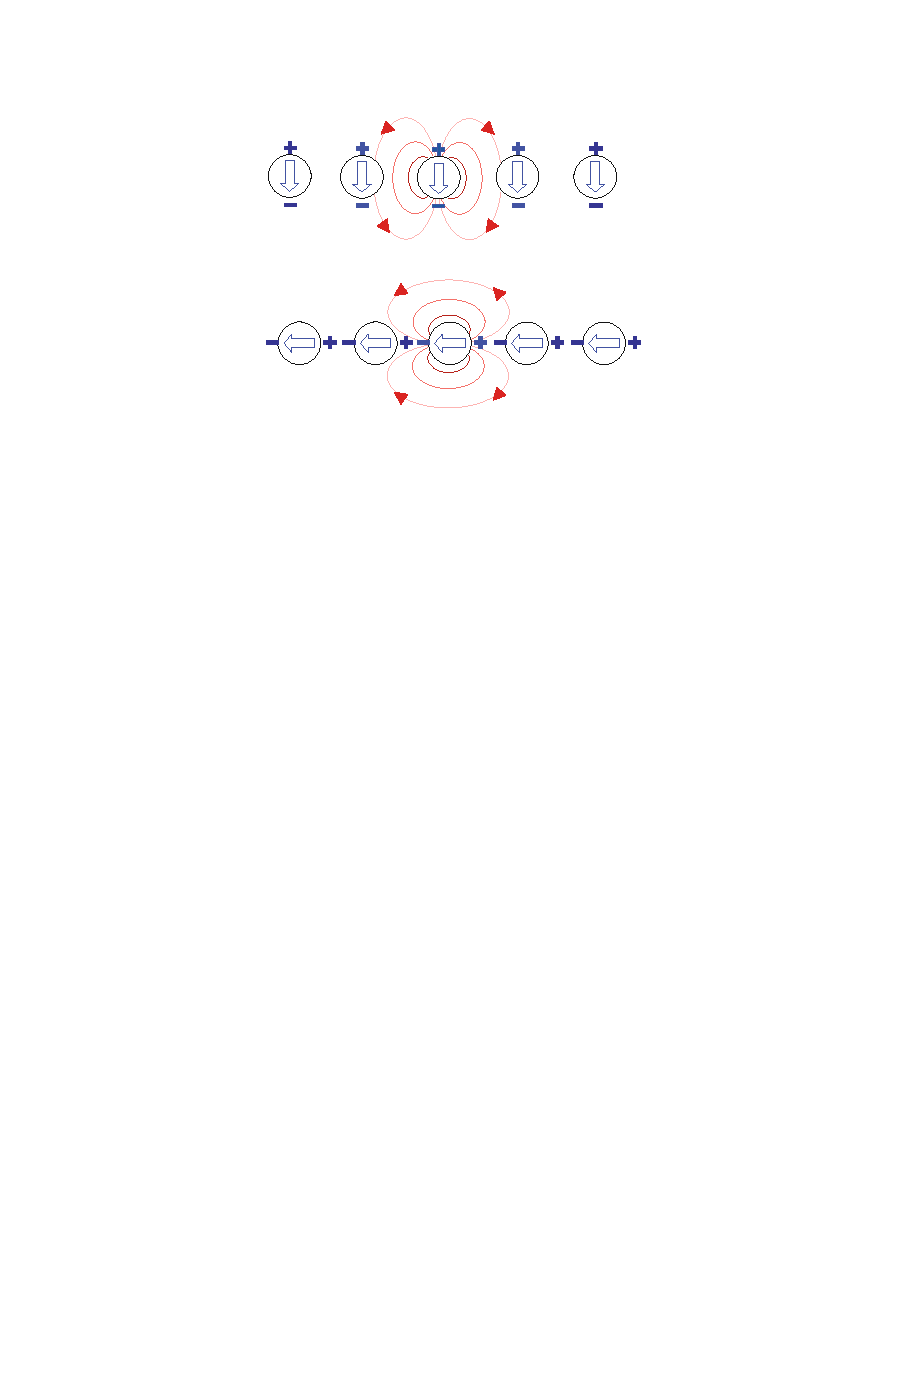
\includegraphics[width=0.45\textwidth]{figures/literature/maier_plasmonics_coupling_diagram}
\quad
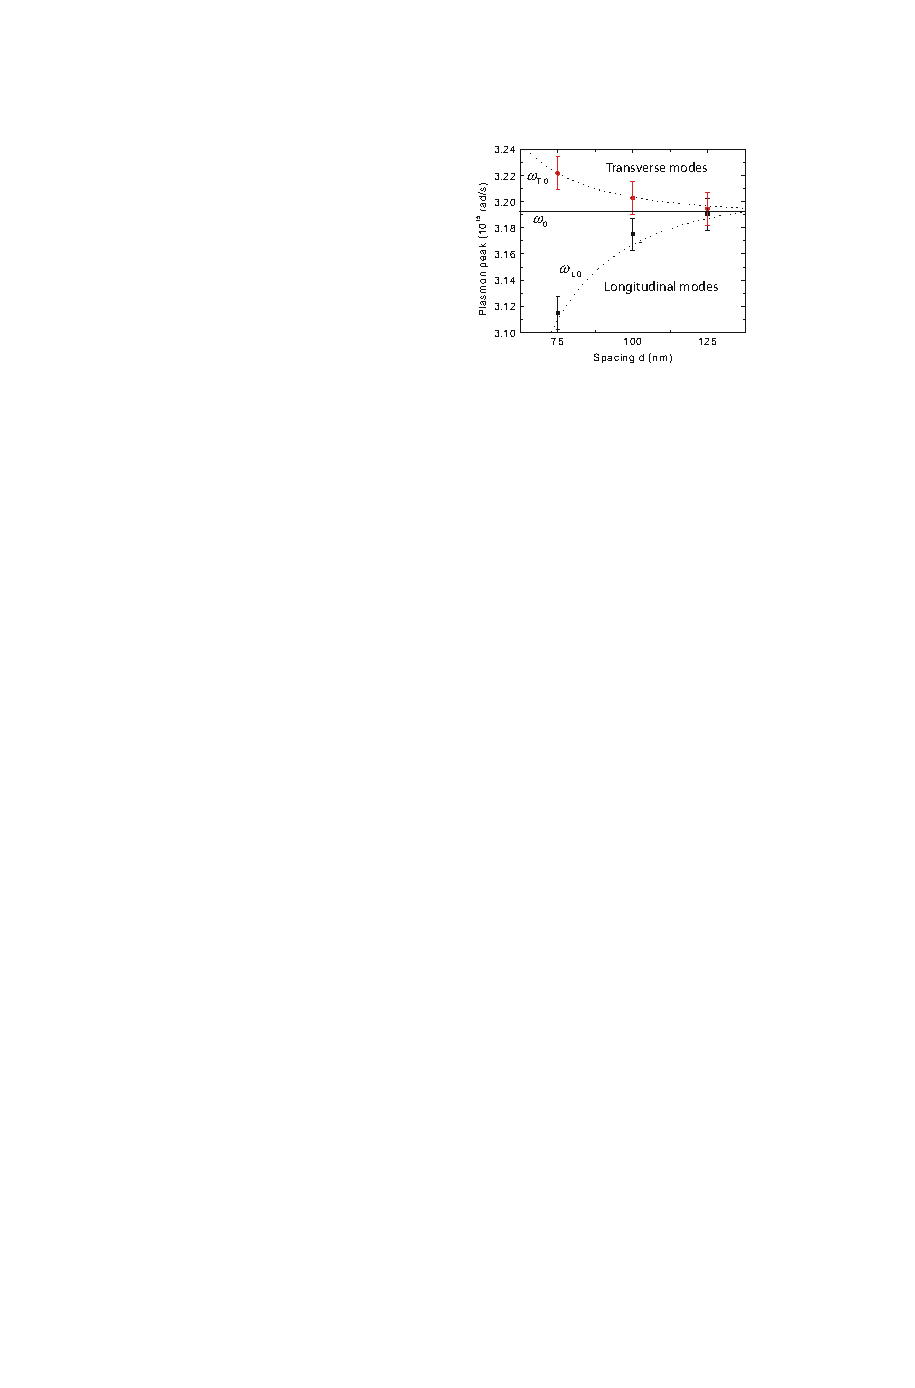
\includegraphics[width=0.45\textwidth]{figures/literature/maier_plasmonics_coupling}
\caption[Experimental and theoretical plasmon coupling]{\textbf{Experimental and theoretical plasmon coupling.} Dipolar plasmons in chains of spherical AuNPs couple depending on field orientation \cite{maier2007plasmonics} (left). Experimentally measured plasmon resonance energies in coupled AuNP chains show the gap-dependent tuning due to coupling \cite{maier2002} (right). The dotted line corresponds to a $d^{-3}$ point dipole model.}
\label{fig:maier_plasmon_coupling}
\end{figure}

In the simplest case, only multipolar plasmons, excited in two isolated spherical \glspl{mnp} being driven by external fields, are considered. This is the prototypical plasmonic dimer system used to understand plasmon coupling. Similar systems, including chains of \glspl{mnp} \cite{maier2002} and \gls{mnp} mirror charges \cite{mertens2013}, have been used to study plasmon coupling.
As the plasmons move closer together the force between charges increases, further polarising the local gap region to which the charge is confined. The introduction of distance-dependent forces to the plasmon oscillator shifts the resonance frequency of the individual plasmon mode from $\omega_0$ by $\Delta\omega$. The coupling strength dictates the extent to which gap plasmon modes deviate from initial plasmon resonances. Since coupling is between multipolar fields, the relative orientation between the particles and the external driving field is important to determining the normal modes of oscillation, along with the phase of the driving field across the \gls{mnp} system. Coupling is strongest when adjacent plasmon poles are oppositely charged.

% Field enhancement increase
The primary {\color{red}result/effect} of gap plasmon excitation is the localisation of electric field to the dielectric medium. As stated previously, a plasmon intrinsically enhances the near-field around a metallic particle, caused by {\color{red}the optically-driven} charge accumulation at the metal-dielectric interface. For the case of two interacting plasmonic particles, the forces between plasmons pulls charge more towards the region between particles. As a result charge accumulates on the metal surfaces around the gap.
Much like with charged plates in a capacitor, the field in the dielectric region greatly increases.
This increase in charge density from the initial plasmon field distribution further increases the near-field enhancement but on a much more confined length scale. For a strongly confined gap mode there is very little field in the metal with almost all field confined within a small lateral mode within the gap. This is known as a plasmonic "hot spot". Through this mechanism {\color{red}alone} the field enhancement $\left|E/E_0\right|$ can be increased from $\sim 5$ to up to $\sim 100$. For this reason attention has shifted from individual plasmonic nanostructures to coupled systems to extract the maximum performance.
\footnote{Is charge localisation only for the in-phase bonding modes via attraction since the other modes are from repulsion?}

% Experimental evidence
Systems of AuNPs were studied from 2003 \cite{maier2002}, in which the individual resonances of AuNP chains with different spacings were shown to couple and form two new modes gradually separating in energy with increased coupling strength (\figurename~\ref{fig:maier_plasmon_coupling}). These modes are the in-phase coupled modes between particles in orthogonal polarisations. The resonance along the chain redshifts with increased coupling due to attraction between plasmons whereas the resonances perpendicular to the chain blueshift as dipolar plasmons in this orientation repel.

\begin{wrapfigure}{O}{0.35\textwidth}
\vspace{-10pt}
\fontsize{10pt}{1em}\selectfont
\def\svgwidth{\textwidth}
\subimport{./figures/}{dipole_interactions.pdf_tex}
\caption[Diagram of dipole interactions]{\textbf{Diagram of dipole interactions.} Dipoles have length $D$. The distance between dipoles is $d$ with an edge-to-edge separation $s$. Configurations 1 and 3 are comparable with plasmon coupling as a result of sub-wavelength structures being driven by a single external light field. Configurations 2 and 4 are generally unphysical without significantly increasing the system size.}
\label{fig:dipole_interactions}
\vspace{-5pt}
\end{wrapfigure}

Interactions between plasmons appear similar to dipole-dipole interactions, which also depend on separation and relative orientation. Examples of dipole-dipole spatial interaction geometries are shown in \figurename~\ref{fig:dipole_interactions}. For two parallel dipoles aligned along their axes, driven in phase, (configuration 1) the attractive coupling potential increases with decreasing separation, $d$, as $V \propto p_1p_2d^{-3}$ \cite{halas2011}. For an oscillating dipole this decreases the resonant frequency. Conversely, the repulsive interaction between two parallel dipoles aligned perpendicular to their axes (configuration 3), also increasing as $d^{-3}$, but increases the resonant frequency. Symmetric anti-phase configurations lead to local field cancellation. Observation of such modes only become possible in non-symmetric dipole-dipole systems once a system become large enough that phase retardation of the driving field is significant.

For plasmons in \glspl{mnp}, the coupling interaction is well approximated using the dipole-dipole model \cite{kreibig1995optical, maier2002, gluodenis2002, rechberger2003}, however the restoring force within the particles also contributes to the potential and goes as the volume $D^3$. The interaction energy between two plasmons therefore goes as $(d/D)^{-3}$. Since the gap size, $s=d-D$, is the defining feature of a plasmonic dimer, relations are often expressed in the quantity $(s/D) = (d/D)-1$ rather than using the centre of mass separation. The resonant wavelength shift due to coupling can then be described using a plasmon ruler equation \cite{jain2007, ben2011},
\begin{equation}
\frac{\Delta\lambda}{\lambda_0} = a\exp\left(-\frac{(s/D)}{\tau}\right),
\label{eq:plasmon_ruler}
\end{equation}
where $a$ is the couple strength and $\tau$ is a decay constant. The exponential decay is considered to be approximately equivalent to the $(s/D)^{-3}$ behaviour, which is expressed in terms of shape and size parameters, $\Lambda$ and $\gamma$, as,
\begin{equation}
\frac{\Delta\lambda}{\lambda_0} = \frac{1}{12\Lambda(s/D+1)^3 - (1-\gamma)}.
\end{equation}
In recent years this relation still shows good agreement with experimental data \cite{} but the approach remains limited to describing only dipolar modes in simple geometries.

% Plasmon hybridisation theory
\begin{figure}[bt]
\centering
\fontsize{10pt}{1em}\selectfont
\def\svgwidth{0.98\textwidth}
\subimport{./figures/}{plasmon_dimer_hybridisation.pdf_tex}
\caption[Diagram of plasmon hybridisation between coupled plasmons in a nanoparticle dimer]{\textbf{Diagram of plasmon hybridisation between coupled plasmons in a nanoparticle dimer.} Plasmons are coupled along the dimer axis. Coupling leads to bonding and anti-bonding modes for each set of interacting $l$ modes. Interaction with higher order $l$ modes lowers the overall energy of lower order coupled modes (green lines). Only the bonding ($\omega_{\uparrow\uparrow}$) mode in the symmetric (homo-)dimer has a net dipole moment and is therefore observable. Cancellation of the net dipole moment means the anti-bonding ($\omega_{\uparrow\downarrow}$) mode remains optically dark. On the contrary, asymmetry in a (hetero-)dimer means both modes stay bright with the lower and higher energy individual modes forming the bonding and anti-bonding hybridised modes, respectively. This diagram is adapted from \cite{nordlander2004}.}
\label{fig:plasmon_hybridisation}
\end{figure}

A slightly more complex model explaining the formation and behaviour of coupled modes was developed between 2003 and 2004. Plasmon hybridisation describes the plasmon resonances of a complex particle geometry by deconstructed it into two simpler geometries \cite{prodan2003, prodan2004}. This is done in analogy with the ideas underpinning molecular orbital hybridisation and the hybridisation of quantum energy states. Using this logic, the theory equally describes the plasmon resonances of two coupled simple particle geometries \cite{nordlander2004} or a particle coupled with its image charge in a surface \cite{nordlander2004a}. The multipolar modes of the individual dimer particles split in energy into two hybridised modes representing the bonding (in-phase) and anti-bonding (anti-phase) pole configurations. Due to the attractive and repulsive nature of the bonding and anti-bonding configurations the coupled modes redshift and blueshift from the initial mode position, respectively. This behaviour is shown in \figurename~\ref{fig:plasmon_hybridisation}.

% bonding vs anti-bonding
This model clearly shows that the bonding and anti-bonding modes have very different radiative properties. The bonding dipole exhibits a large net dipole moment due to the parallel alignment of individual dipoles, whereas the anti-parallel aligned anti-bonding mode has no net dipole. As a result, the bonding mode strongly couples with light whereas the anti-bonding mode remains dark. Consequently, anti-bonding modes can be referred to as dark modes. They only become visible once a net dipole moment becomes possible, either through asymmetry of the dimer particles (difference material, size or shape) or once dimer particles become large enough that phase retardation can vary the relative dipole amplitudes.

% mixing of different l modes
Hybridisation between two $l=i$ modes is also influenced by the presence of other modes of $l\neq i$, as is shown by the second set of dashed lines in \figurename~\ref{fig:plasmon_hybridisation}. For most simple dimer systems only the $l=1$ mode is observed, however, with small gaps or large particles, the $l=2$ mode becomes observable. In this case the $l=1$ mode undergoes an increased rate of redshifting due to interaction with the appearing $l=2$ mode. If the gap size becomes small enough that the bonding $l=2$ mode redshifts near to the anti-bonding $l=1$ mode, the interaction decreases the $l=1$ state energy to the point at which the blueshift is reversed \cite{nordlander2004}. Furthermore, should the gap size parameter $s/D$ become even smaller, the increased axial dimer coupling strength means there is the potential to see even higher order modes. Classically, for nm-size gaps, a whole range of higher order modes is expected to exist in the gap \cite{romero2006}. The lateral confinement of these modes across the gap is {\color{red}estimated} using,
\begin{equation} w = \sqrt{Rs}. \end{equation}

% polarisation effects
Only the case of light driving plasmons along the dimer axis is shown in \figurename~\ref{fig:plasmon_hybridisation}. When light drives plasmons perpendicular to this axis the coupling strength is reduced and the excited plasmon poles repel each other. The bonding mode in this polarisation then blueshifts with increased coupling \cite{gunnarsson2005}.

% Mixing of gap modes with antenna modes

\subsection{Charge Transfer Plasmonics}

% Plasmonics on geometrical contact
\begin{figure}[bt]
\centering
\fontsize{10pt}{1em}\selectfont
\def\svgwidth{0.65\textwidth}
\subimport{./figures/}{plasmon_contact.pdf_tex}
\caption[Diagram showing the emergence of charge transfer and screened bonding (crevice) plasmons on geometrical contact in a nanoparticle dimer]{\textbf{Diagram showing the emergence of charge transfer and screened bonding (crevice) plasmons on geometrical contact in a nanoparticle dimer.} The field generated by the bonding dimer plasmon (BDP) is screened from the gap by the conductive contact, forcing capacitive coupling to the crevice gap in the form of the screened bonding dimer plasmon (SBDP). The dominant charge oscillation is then the charge transfer plasmon (CTP) through the conductive bridge and across the whole structure.}
\label{fig:plasmon_contact}
\end{figure}

Upon geometrical contact between particles in a \gls{mnp} dimer the gap becomes a conductive bridge. If its length is small and its conductivity is high such that charge can be transported between particles within half an optical cycle then \glspl{ctp} can form. The conductive short prevents the accumulation of surface charge on the gap-facing metallic interfaces, reducing the capacitive coupling between plasmons. The capacitive hybridised gap modes are screened by the charge in the gap region and the modes move to the crevice. In another sense there are a finite number of electrons, each in a specific state, therefore if one electron transitions into a collective \gls{ctp} oscillation then it's contribution is lost from it's original capacitive mode.
%
%As discussed in section \ref{sec:em_waves} and shown in \eqref{eq:dielectric_conductivity}, the local conductance around a plasmon is important in determining its properties. The real part of the local conductivity $\sigma$ sets the damping {\color{red}(screening)} ($\real{\sigma(\omega)}\rightarrow\imag{\eps(\vec{k}, \omega)}$) and hence broadening of the plasmon whilst the imaginary part influences the position of the resonance by modifying $\real{\eps(\vec{k}, \omega)}$.
%
Theoretical calculations of this transition from bonding to charge transfer modes have been carried out \cite{romero2006, perez2010, tserkezis2014} with experiments confirming the behaviour \cite{lassiter2008, herrmann2014, benz2014}. Mostly this work has been done using spherical \gls{mnp} dimers, for both numerical and lithographic (experimental) simplicity.

% Classical physics first
Classical physics suggests that upon geometrical contact \gls{ctp} modes form at lower energies than the bonding modes and blueshift as the particles continue to overlap \cite{romero2006}. This occurs since the separation of the poles of \gls{ctp} charge distribution continually decreases, thus increasing the dipole energy. Each bonding mode has a corresponding \gls{ctp} mode.%
\footnote{For a spherical \gls{mnp} dimer with bonding hybridised dipolar (BDP) and quadrupolar (BQP) modes the corresponding CTP modes are typically labelled as CTP and CTP$^\prime$.}
The width of the remaining screened bonding resonances increases due to conductive losses in the mode. As discussed in section \ref{sec:em_waves} and shown in \eqref{eq:dielectric_conductivity}, a new contribution to conductivity will change the dielectric function. The real part of the conductivity $\sigma$ sets the damping {\color{red}(screening)} ($\real{\sigma(\omega)}\rightarrow\imag{\eps(\vec{k}, \omega)}$),  therefore broadening the plasmon resonance, whilst the imaginary part influences the position of the resonance by modifying $\real{\eps(\vec{k}, \omega)}$. A larger overlap means a larger junction conductance, which, along with the geometrical changes, severely changes the optical response of the gap.
The notion of a continually overlapping dimer is mostly unphysical but blueshifting modes back to those of a single isolated sphere is an obvious outcome. This behaviour has been observed experimentally by lithographically creating overlapped discs \cite{lassiter2008}.

% Screening effect
Changeover from capacitive to conductive modes occurs in two steps \cite{perez2010}. First the charge in the gap screens the bonding modes. This occurs for low conductances. An estimate of the conductance threshold for a gap separation $d$ and {\color{red}link/bridge} radius $a$ is,
\begin{equation}
G_{\mathrm{SBDP}} = \frac{\omega_{\mathrm{BDP}}}{2\pi}\frac{a^2}{d}.
\end{equation}
This quantity is considered independent of junction geometry and depends only on the conductivity ($\sigma_{\mathrm{SBDP}} = \omega_{\mathrm{BDP}}/2\pi^2$). For a larger contact width or smaller gap size the threshold is increased to overcome the increased capacitive coupling.
% CTP effect
A second threshold exists for \gls{ctp} formation. For a particle of radius $R$, this occurs at the second threshold,
\begin{equation}
G_{\mathrm{CTP}} = \frac{\omega_{\mathrm{CTP}}}{4\pi}\frac{R^2}{d}.
\end{equation}
In a similar manner to screening the conductivity threshold is expressed as $\sigma_{\mathrm{CTP}} = (\omega_{\mathrm{CTP}}/4\pi^2) (R/a)^2$. Unlike screening, CTP formation depends on not only the conductivity but the junction geometry. The geometry factor $(R/a)$ represents the ratio between the total charge in the particle and that which can pass through the gap at fixed conductivity. Having a large conductivity means the junction does not have to be as wide relative to the particle size to accommodate sufficient charge flow to maintain a \gls{ctp} mode.
% Experimental limitations
It is typically difficult to experimentally correlate these two behaviours as the screened bonding plasmons and \glspl{ctp} are usually separated by a frequency gap larger than the measurable bandwidth of the spectrometer used.

A distinction can be made between systems in which the conductive gap medium is a fixed spacer material whose conductivity can effectively be changed and systems in which the junction has the same conductivity as the metal nanoparticles (approaching nanoparticles) where geometrical changes are the cause for charge transfer phenomena.
% Gap reduction and overlap
Reduction of the gap separation leading to eventual overlap
% Bridging effects
In other instances the gap size has been experimentally fixed, typically using molecules which have a finite conductivity. Connecting AuNPs separated by \SI{0.9}{nm} together with Au bridges using ultrafast laser pulses showed that \glspl{ctp} form resonances in the NIR, which blueshift with increasing width/conductance \cite{herrmann2014, tserkezis2014}. Longer linked chains consisting of small particles showed more blueshifted \gls{ctp} resonances than shorter chains of larger particles.
% BPT-BPDT transition
Varying the gap conductance using fractional mixing of partially conductive molecules with similarly structured insulating molecules has shown screening and blueshifting of the BDP mode and the emergence of a CTP$^\prime$ mode \cite{benz2014}. In this instance the geometry is fixed and system is therefore conductivity limited. The threshold for this behaviour is estimated as 1\G0.

Signatures of charge transfer plasmons have been observed using Raman scattering \cite{elkhoury2014}.

%Tuning of the optical response using conductive linker molecules with varying conductivities between \glspl{mnp} has been achieved \cite{tan2014, benz2014}.

\subsection{The Optical Response of Plasmonic Dimers}
% \cite{kadkhodazadeh2013} should go in last chapter

\begin{figure}[bt]
\centering
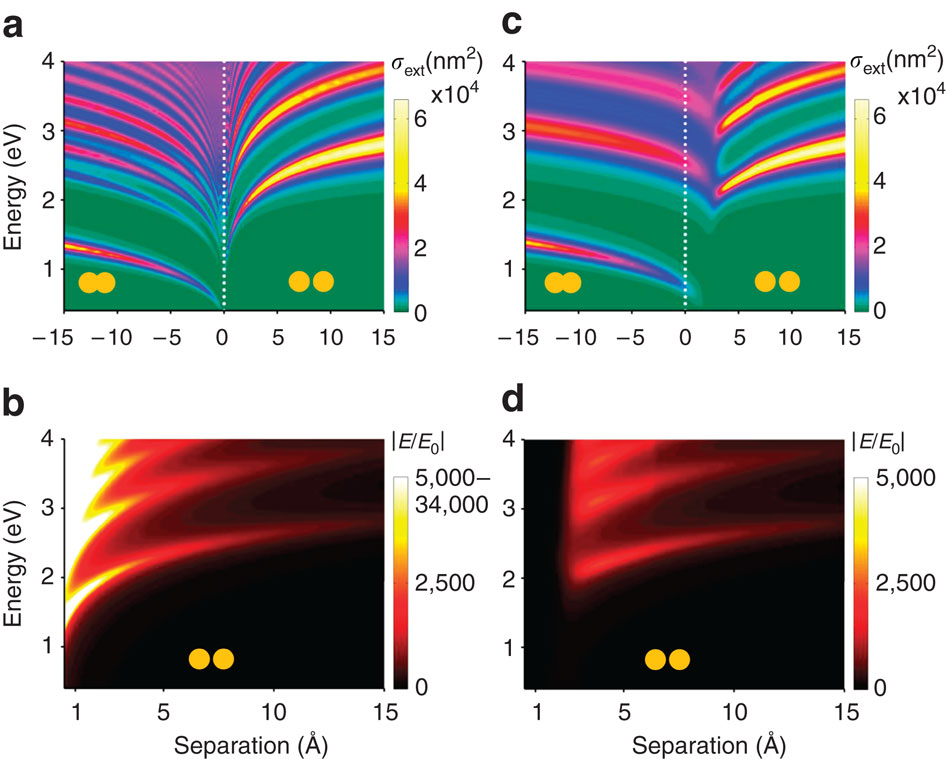
\includegraphics[width=0.7\textwidth]{figures/literature/ncomms1806-f4}
\caption[Numerical calculated extinction cross-section and field enhancement of a spherical AuNP dimer as a function of gap separation \cite{esteban2012}]{\textbf{Numerical calculated extinction cross-section and field enhancement of a spherical AuNP dimer as a function of gap separation \cite{esteban2012}.} The classical approach (left), valid for separations greater than $\sim$\SI{5}{\angstrom}, shows many modes redshifting into a singularity on geometrical contact, following by blueshifting CTP modes as the particles overlap. Introduction of an effective (conductive) gap medium to emulate the effects of quantum tunnelling (quantum corrected model, right) demonstrate the early onset of screening and CTP formation prior to geometrical contact. Figure taken from \cite{esteban2012}.}
\label{fig:optical_response_dimer}
\end{figure}

The full separation-dependent optical response of a plasmonic dimer can be numerically calculated to demonstrate the behaviour of coupled plasmons as the dimer transitions from a non-interacting state through to geometrical contact and eventual overlap of particles \cite{romero2006, esteban2012}.
The lowest order modes in the individual particles redshift and increase in intensity as the separation decreases. Once the gap size becomes even smaller higher order modes appear and redshift. As the higher order modes become more intense scattering from the lowest order modes decreases, despite the field enhancement increasing. These plasmons have become so confined to the gap that they no longer couple with the far-field. This summarises the classical picture of plasmon coupling (\figurename~\ref{fig:optical_response_dimer}a,b).

% Onset of tunnelling
The classical picture description breaks down under two conditions - either the particles become sufficiently small that quantum non-locality and non-local effects (finite, non-negligible electron wavefunction spill-out from the particle) become important or the gap size decreases to scales on which quantum tunnelling can no longer be ignored. The onset of quantum tunnelling means charge is transported across the gap without requiring geometrical contact. The effects of quantum tunnelling were first predicted in small ($R<\SI{2}{nm}$) Na \glspl{np} using full quantum mechanical time-dependent \gls{dft} calculations \cite{zuloaga2009}. Since these calculations consider the behaviour of each electron, they are limited in complexity to small systems containing less than 2000 electrons.

Tunnelling effects in larger metallic nanostructures are predicted by the \gls{qcm}, a classical model which uses an effective gap dielectric function that takes into account quantum effects \cite{esteban2012}. Electron tunnelling is accounted for using pre-calculated conductance parameters as a function of separation from \gls{dft} calculations. For large surfaces and small gaps the integrated contribution to conductance from tunnelling across the gap is enough to initially screen the bonding plasmons followed by the formation of \glspl{ctp} (\figurename~\ref{fig:optical_response_dimer}c,d). Screening leads to strong attenuation of the field enhancement in the gap. The lack of modes present when considering quantum effects is a result of electron tunnelling smoothing the effective junction surface. It should be noted that whilst the bonding mode appears to blueshift as a result of screening reducing the capacitive coupling, simulations suggest that the blueshifting resonance is a higher order \gls{ctp} excitation.

\begin{figure}[bt]
\centering
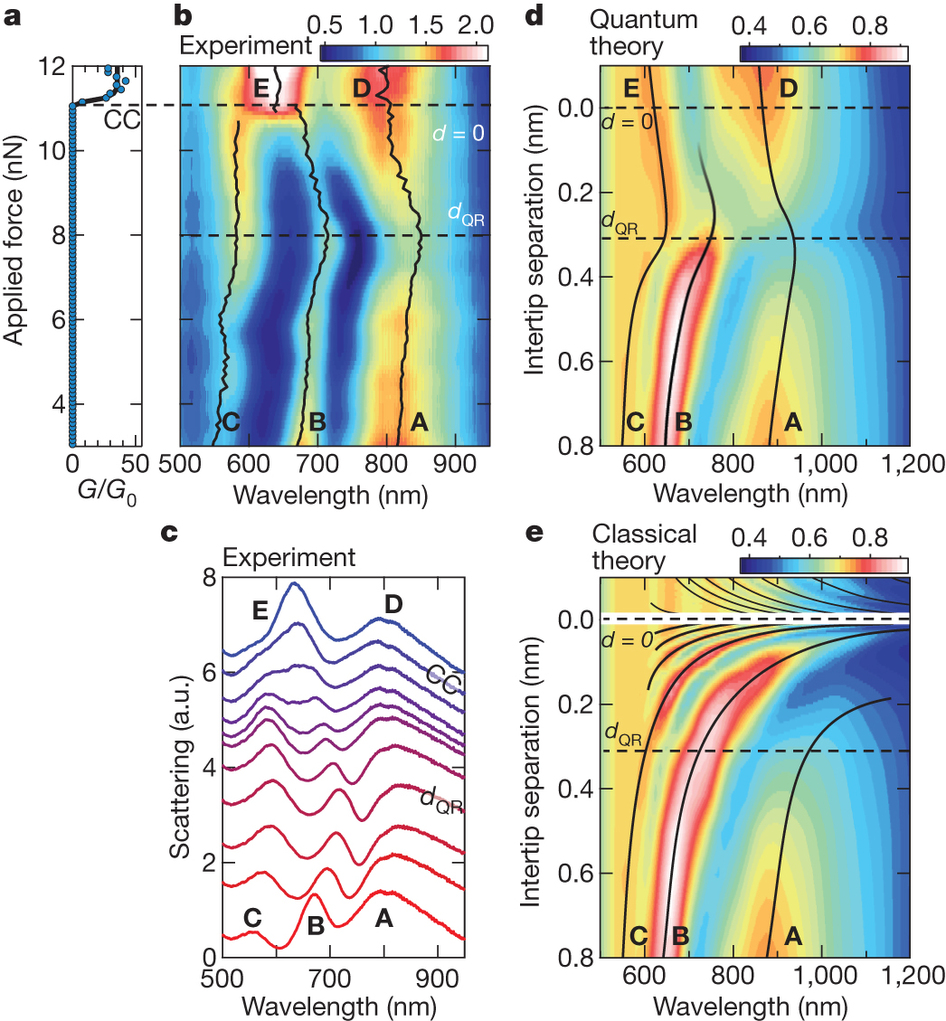
\includegraphics[width=0.65\textwidth, clip=true, trim=0 500 0 0]{figures/literature/nature11653-f2_2}\\
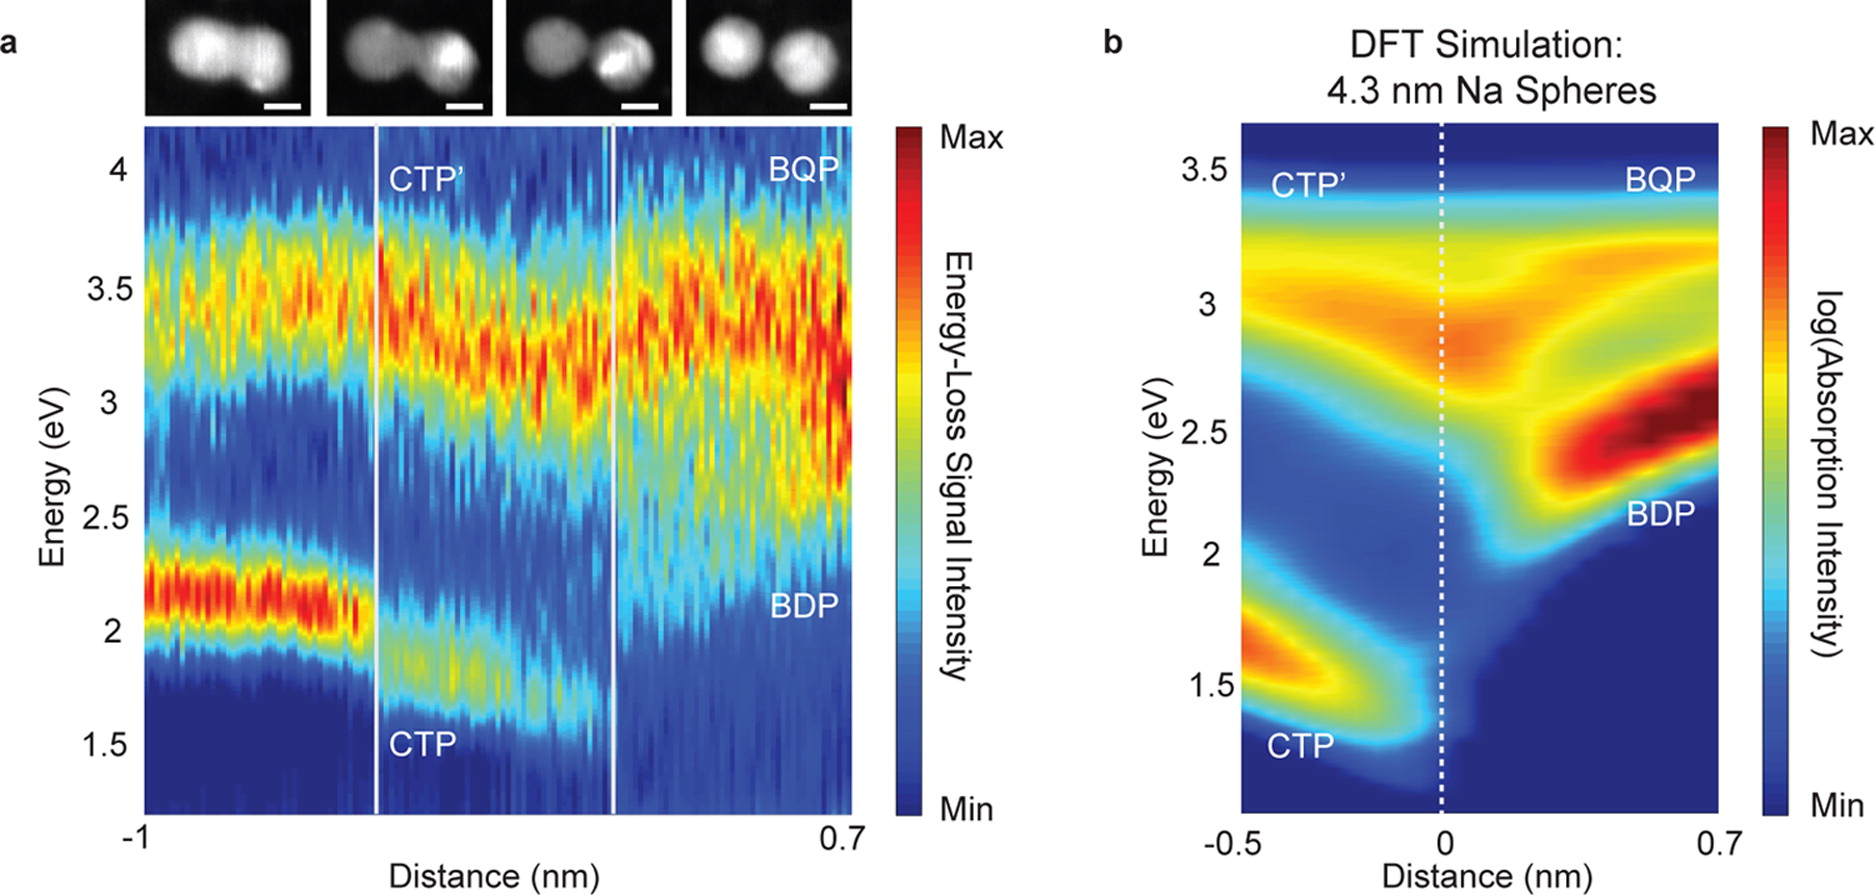
\includegraphics[width=0.65\textwidth]{figures/literature/nl-2012-04078v_0001}
\caption[Examples of experimental measurements of the effect of quantum tunnelling on plasmonic gap systems]{\textbf{Examples of experimental measurements of the effect of quantum tunnelling on plasmonic gap systems through direct monitoring of the plasmon resonances.} (top) Supercontinuum dark-field scattering measurements of two \SI{300}{nm} diameter spherical Au tips in a dimer configuration with reducing separation, transitioning below \SI{1}{nm} and into the quantum regime \cite{savage2012}. (bottom) EELS measurements of \SI{10}{nm} AgNPs being induced closer together by the electron beam \cite{scholl2013}.}
\label{fig:tunnelling_plasmonics}
\end{figure}

% Experimental measurements
Experimental evidence of quantum tunnelling influencing plasmon coupling has been observed using both optical spectroscopy \cite{savage2012, cha2014, zhu2014}, EELS \cite{scholl2013}, SERS \cite{zhu2014}, photoluminescence \cite{kravtsov2014} and third-harmonic generation measurements \cite{hajisalem2014}.
% Direct measurements
First measurements were made using optical scattering from a dynamic spherically-tipped Au AFM probe dimer, with simulated spectra using the \gls{qcm} (\figurename~\ref{fig:tunnelling_plasmonics}) \cite{savage2012}. Plasmon modes are shown to blueshift upon decreasing past a critical separation. Scattering spectra qualitatively agreed with the \gls{qcm}, with discrepancies attributed to difficulty in simulating an extended dual tip geometry. Better agreement with theory was found in EELS measurements on simpler \SI{10}{nm} AgNP dimers, brought together under the influence of the electron beam (\figurename~\ref{fig:tunnelling_plasmonics}) \cite{scholl2013}. EELS agreed very well with \gls{dft} calculations.
% Molecular distance tuning - note this is not the best quality data or papers
Alkanedithiol molecules of various lengths have also been used to discretely tune the gap separation of AuNP dimers \cite{cha2014}. In this case, blueshifting and attenuation of the BDP, as well as a measured increase in its width, is measured with molecules smaller than pentanedithiol. Similar results are found when using intercalating \glspl{sam} \cite{tan2014}.
% Inferred measurements
Further measurements on sub-nm plasmonic gaps have also shown changes attributed to quantum tunnelling, though inferred from properties depending on the gap field enhancement as opposed to direct monitoring of the plasmon resonances. A decrease in signal intensity in both the SERS peaks \cite{zhu2014} and photoluminescence \cite{kravtsov2014} are signatures of quantum tunnelling screening the coupled plasmon field.

\begin{figure}[bt]
\centering
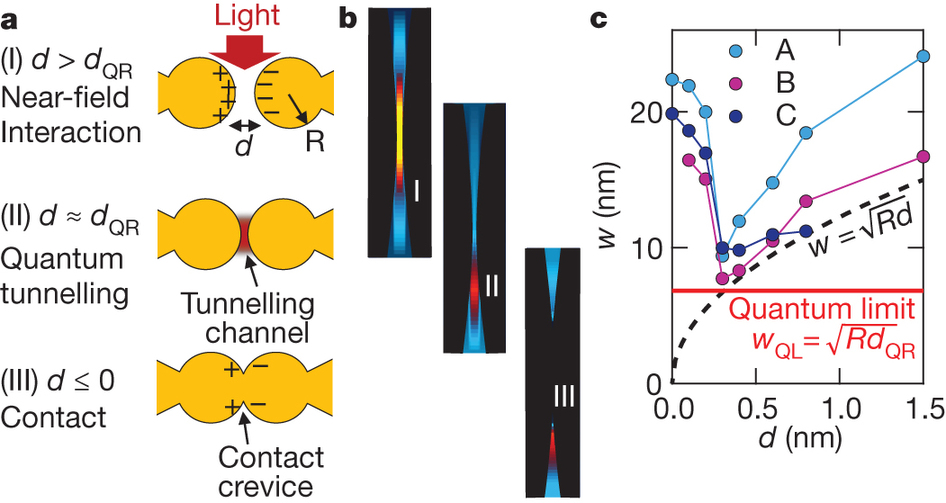
\includegraphics[width=0.6\textwidth]{figures/literature/nature11653-f3_2}
\caption[Plasmon mode distributions in the quantum regime]{\textbf{Plasmon mode distributions in the quantum regime.} Diagram showing the different regimes of plasmonic interaction, taken from \cite{savage2012}. The onset of a tunnelling current pinches of the electric field in the gap via screening/conductive losses prior to conductive contact, which shows a similar expulsion of field from the gap.}
\label{fig:savage2012c}
\end{figure}

Interestingly, qualitative (and to some extent quantitative) agreement between \gls{qcm} calculations and full quantum calculations suggest that the quantum nature of the system is of little importance. Despite only using a classical, resistive gap with conductances given by values characteristic of electron tunnelling, the effect of electron tunnelling on gap plasmons is accurately replicated. This implies that the effects on the plasmons, despite the quantum nature of electron tunnelling, depends only on the amount of charge transfer and not the mechanism by which it occurs. This links together work done using particle positioning \cite{savage2012, scholl2013} with studies of interacting plasmonic system coupled with molecular linkers \cite{tan2014, benz2014, cha2014}.

Quantum tunnelling still remains an interesting case, however, since it is a form of conduction that is unavoidable once system sizes decrease below \SI{0.5}{nm}. This is why its pinch-off point, the point at which the electric field in the gap is expelled, is described as the quantum limit to plasmon confinement \cite{savage2012}. It is for this reason why it is important to fully understand the relations between plasmonic hot-spots and sites of (quantum) charge transfer.

\end{document}